\newcommand{\component}[1]{\textbf{#1}}
\newcommand{\componentlabel}[1]{\textbf{#1}}

\section{Execution}
\label{sec:durchfuehrung}
This section describes the experimental setup as well as the procedure to be followed.

\subsection{Setup}
% - laser construction
%   - diode laser
%     - knobs: TOP / SIDE
%   - collimating lens
%   - grating
%     - piezo
% - absorption cell
%   - Rb
%   - heated to 50 °C
% - 50/50 mirror, filters…
% - IR viewing card
% - CCD camera + monitor
% - control unit
% - oscilloscope

The laser apparatus consists not only of the laser diode,
but also components for wavelength selection, angular alignment and temperature control.
A collimating lens directs the highly divergent laser beam to a reflective grating,
whose first order interference maximum feeds back into the laser,
thus creating an \component{external cavity}.
The angle of the grating (which has vertically oriented grooves)
is adjusted using the \componentlabel{TOP} and \componentlabel{SIDE} knobs.
While the \componentlabel{TOP} knob rotates the grating about an axis parallel to the optical table and perpendicular to the incoming beam,
    thus changing the length of the \component{external cavity},
the \componentlabel{SIDE} knob rotates the grating about an axis perpendicular to the optical table,
    which additionally changes the wavelength of the constructive interference that goes back into the laser.
    % resulting in a change in the angle relevant for interference in addition to changing the cavity length.
In addition to the \componentlabel{SIDE} knob,
a \component{piezo stack} allows for fine-tuning and quick sweeps.
%
The rubidium
    whose spectrum is to be analyzed
is located in an \component{absorption cell} that is
    heated to \SI{50}{\celsius} and
    positioned after the zeroth order intensity maximum of the grating.
%
For the last part of the experiment,
a \component{50/50 beam splitter} and various \component{neutral-density filters} are available.
An \component{IR viewing card} as well as a \component{CCD camera} connected to a \component{monitor}
facilitate the adjustment of the otherwise (especially when wearing eye protection) invisible laser beam.
%
A \component{control unit} provided by TeachSpin contains all the necessary electronics
    to control the laser and the \component{absorption cell}
    as well as to measure the spectrum.
In particular,
it contains a ramp generator
    that will be used for scanning the wavelength of the laser
and a differential amplifier
    for measuring the absorption of the rubidium without disturbance. % COULDDO: phrasing
%
Finally, an oscilloscope displays the monitor signals of the detector circuit and ramp generator.


\subsection{Procedure}
% COULDDO: Mention: Check that the laser current is set to 0.
    Assuming the main components are already connected and positioned on the optical table,
once the environmental light is dimmed and everyone in the room wears eye protection,
the \component{control unit} may be powered on.
The integrated temperature controller will begin heating the \component{absorption cell} to \SI{50}{\celsius}
in order to increase the rubidium vapor density and thus the absorption.


\subsubsection{External Cavity Alignment}
For the first procedure,
% NOTE: The instructions ask us to use a blank business card instead. I don't think it matters much.
the \component{IR viewing card} is placed in a holder
and the \component{CCD camera} is positioned in a way that the (indirect) image of the laser spot will visible on the monitor,
as shown in \autoref{fig:schematic1}.

The laser current is then slowly increased until the beam shows.
At a certain point the beam's intensity will increase rapidly,
and speckles (random interference patterns) will appear.
This is the point where the laser actually starts to lase monochromatically instead of behaving like an LED (see \autoref{sec:theorie}). % COULDDO: too casual?
Said current is written down for future reference.
For currents slightly below as well as slightly above the threshold,
a photo is taken.
The current is left slightly above the threshold.

For vertical alignment, the \componentlabel{TOP} knob (see \autoref{fig:knobs}) is carefully turned,
which may be facilitated by using an Allen wrench.
As the laser goes through the longitudinal modes defined by the length of the external cavity,
a periodic variation of its intensity can be observed.
For optimal results in the next steps,
an intensity maximum near the center of these mode maxima is chosen.

% NOTE: The TOP knob does not change the wavelength that's reflected back into the laser,
% because it rotates the grating on an axis parallel to the optical table.

\begin{figure}
    \centering
    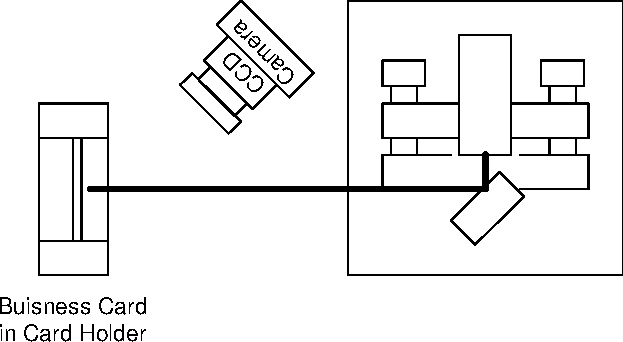
\includegraphics[width=0.5\textwidth]{content/img/p30_Fig1.pdf}
    \caption{Schematic of the experimental setup for aligning the external cavity \cite{versuchsanleitung}.}
    \label{fig:schematic1}
\end{figure}

\begin{figure}
    \centering
    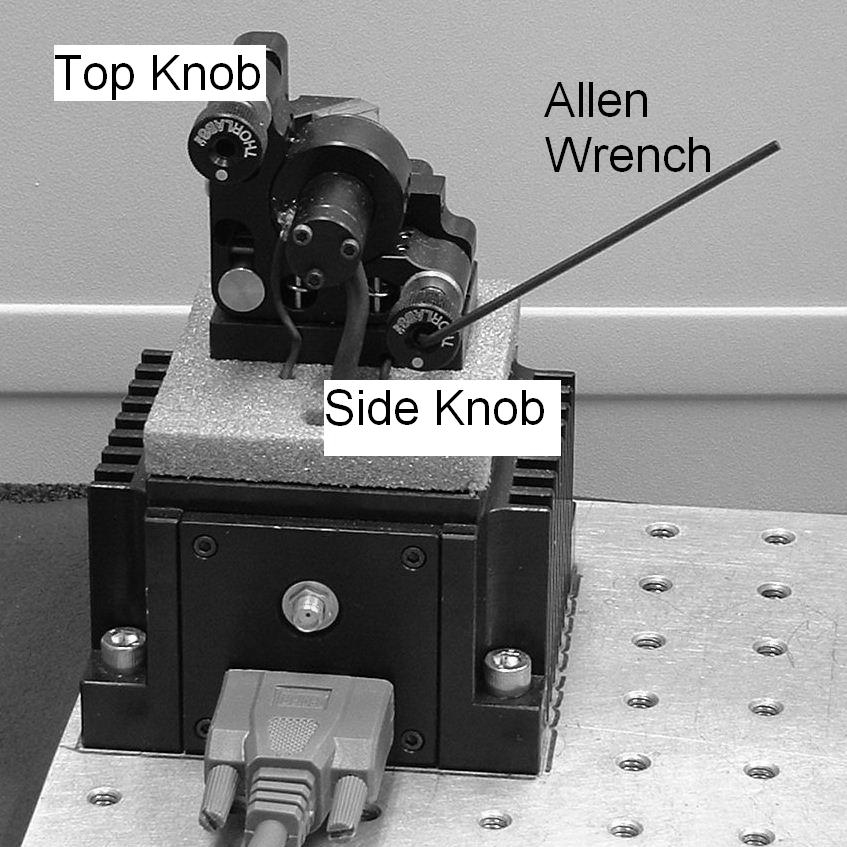
\includegraphics[width=0.5\textwidth]{content/img/p31_Fig2.png}
    \caption{Labeled image of the laser apparatus and its adjustment knobs \cite{versuchsanleitung}.}
    \label{fig:knobs}
\end{figure}


\subsubsection{Preparation for Observing Rubidium Fluorescence}
As the next step,
the laser is further tuned to the \ce{Rb} absorption lines.
For this,
the \component{IR viewing card} is removed and optionally placed behind the \component{\ce{Rb} cell},
which is located on the optical axis.
The camera is then repositioned to record the inside of the \component{absorption cell} through the \component{Side Hole}.
A schematic of the new arrangement is given in \autoref{fig:schematic2}.
Now the \component{Ramp Generator} is enabled and set to a low frequency (\SI{10}{\hertz}) to drive the piezoelectric stack,
which will move the grating according to a triangle wave in order to scan the laser wavelength.
\autoref{fig:wiring2} shows the necessary wiring.
To ensure correct operation,
the oscilloscope can be connected to
    the \componentlabel{SYNC OUTPUT} of the \component{Ramp Generator} and
    the \componentlabel{MONITOR OUTPUT} of the \component{Piezo Controller}.
% NOTE: We were told that also modulating the current in this step could make things easier.

Assuming sufficient previous calibration,
the camera monitor should show the rubidium fluorescence as a ray of light,
pulsing at the previously set frequency.
% COULDDO: Doofer Satz ↓
By carefully adjusting the \componentlabel{SIDE} knob (see \autoref{fig:knobs}),
the wavelength of the laser is roughly selected,
% which means the piezo stack is only used for sweeping and fine-tuning
adding to the piezo stack's fine-tuning
and therefore reducing the need for high offset voltages.
% NOTE: The instructions state that that the flourescence is always visible.
% But the pulsing shouldn't stop, because even in the range we want to measure, only the absorption lines should result in fluorescence.
The knob is turned until the fluorescence is always visible.
Then, the laser current is varied to maximize its intensity.

\begin{figure}
    \centering
    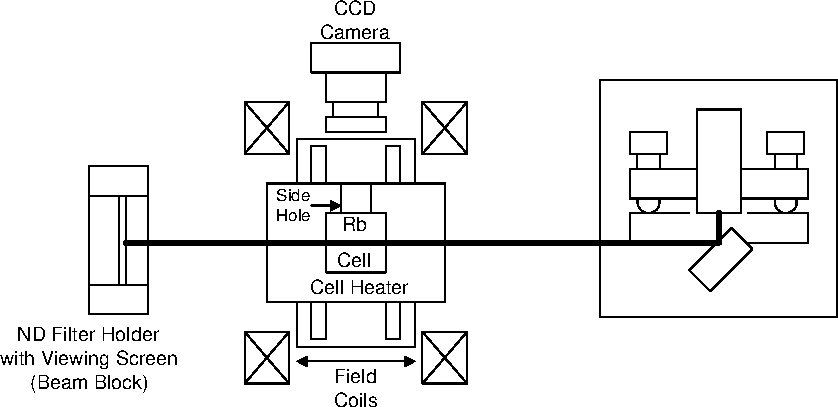
\includegraphics[width=0.75\textwidth]{content/img/p33_Fig4.pdf}
    \caption{Schematic of the experimental setup for finding the \ce{Rb} fluorescence \cite{versuchsanleitung}.}
    \label{fig:schematic2}
\end{figure}

\begin{figure}
    \centering
    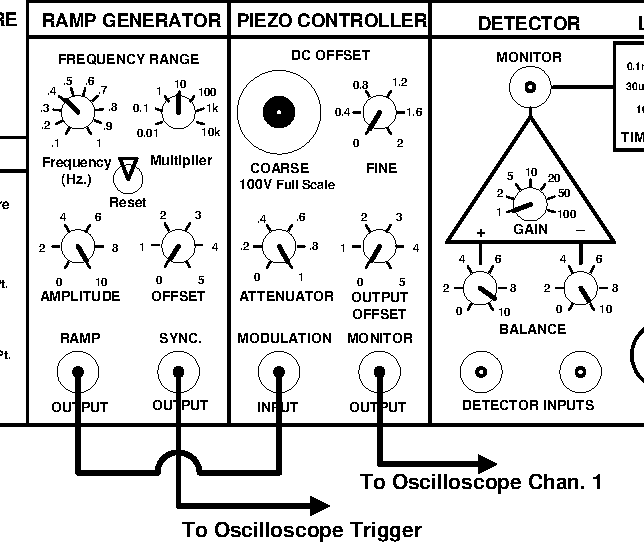
\includegraphics[width=0.75\textwidth]{content/img/p34_Fig5.pdf}
    \caption{Wiring diagram of the control unit while searching for the \ce{Rb} fluorescence \cite{versuchsanleitung}.}
    \label{fig:wiring2}
\end{figure}


\subsubsection{Observation of the Absorption Spectrum}
% Using Simultaneous Current and Piezo Modulation to produce a larger scan range without mode hops.
% Using Two Photodiode Detectors to Compare a Beam directly from the Laser to one that has passed through rubidium vapor

In order to eliminate \hyperref[sec:theorie:modehops]{mode hops} and cover the entire frequency range of interest,
not only the position of the external (cavity) modes need to be modulated (via the grating / piezo stack as before),
but also that of the internal modes.
This is accomplished by additionally modulating the laser current.

Since the laser current directly affects its intensity,
the absorption spectrum measured by a single \component{photodiode detector} behind the \component{\ce{Rb} cell} would be skewed.
To avoid this,
only the difference in intensity is considered:
A \component{50/50 Mirror} is placed in the optical path,
directing half of the laser beam to a second \component{photodiode detector},
while the other half passes through the \component{\ce{Rb} cell} and is detected by the first \component{photodiode detector}.
\component{ND Filters} might need to be added after the laser to prevent saturation of the photodiodes.
In \autoref{fig:schematic3}, the new arrangement is shown.
The \component{Control Unit} contains a differential amplifier with adjustable gain and balance of the two signals.
Its output is connected to the \component{oscilloscope},
which should now show the expected absorption spectrum of the \component{\ce{Rb} cell}.
\autoref{fig:wiring3} shows the updated wiring.

After observing the photodiode signals individually,
the differential amplifier is set up to yield the best possible signal.
For a last time,
    the base laser current,
    the piezo's \componentlabel{DC offset}, % Oxford comma
    and the \componentlabel{SIDE} knob
are optimized,
before a screenshot of the oscilloscope is taken.

\begin{figure}
    \centering
    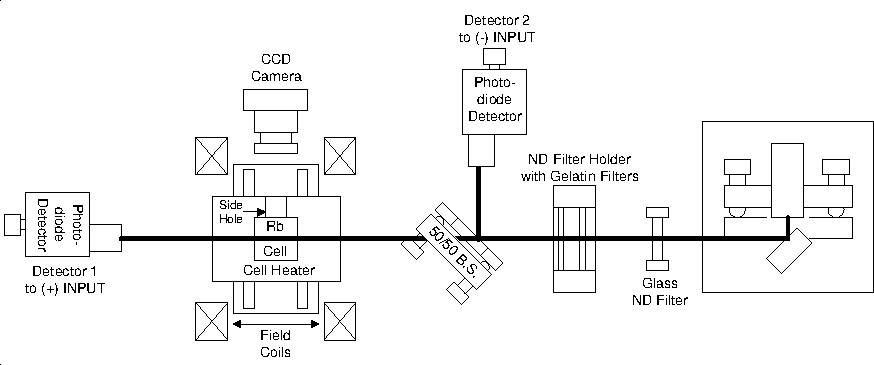
\includegraphics[width=0.75\textwidth]{content/img/p40_Fig12.pdf}
    \caption{Schematic of the experimental setup for measuring the \ce{Rb} fluorescence \cite{versuchsanleitung}.}
    \label{fig:schematic3}
\end{figure}

\begin{figure}
    \centering
    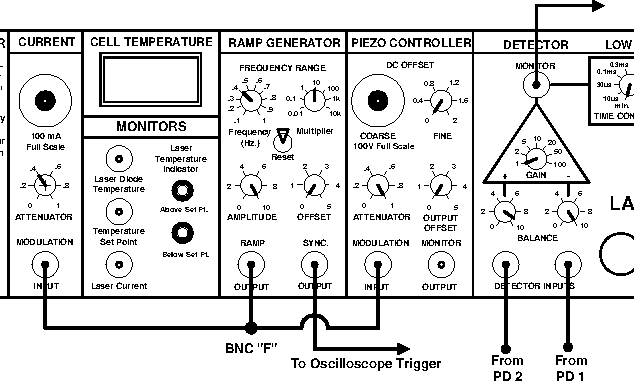
\includegraphics[width=0.75\textwidth]{content/img/p40_Fig13.pdf}
    \caption{Wiring diagram of the control unit while measuring the \ce{Rb} fluorescence \cite{versuchsanleitung}.}
    \label{fig:wiring3}
\end{figure}
